%@TheDoctorRAB
%
%presentation template for class slides and research presentations
%allows for citations in slide and a list at the end
%
%%%%%
%
%REFERENCES
%
%neup.bst - numbered citations in order of appearance, short author list with et al in reference section
%nsf.bst - numbered citations in order of appearance, full author list in references section
%standard.bst - citations with author last name with et al for more than 2 authors; full author list in references section
%ans.bst is for ANS only. 
%
%author = {Lastname, Firstname and Lastname, Firstname and Lastname, Firstname} for all bst formats
%bst renders the author list itself
%
%author = {{Nuclear Regulatory Commission}} if the author is an organization, institution, etc., and not people
%
%title = {{}} for all
%
%for all - use \citep{-} - [1] or (Borrelli, 2021) in the text
%standard.bst \cite{-} - Borrelli (2021) in the text
%standard.bst lists references alphabetically
%the rest list numerically
%
%
%%% citations on slides 
%
%\citep{xxxnna} where the citation should go
%\blfootnote{\fontsize\cite{xxxnna}\fontsize\bibentry{xxxnna}} before \end{frame}
%
%
%%%%%

%%%%% presentation settings
\documentclass[aspectratio=1610,pdftex,dvipsnames,compress,xcolor={dvipsnames}]{beamer}
\usetheme{Boadilla}
\usecolortheme{seahorse}
\beamertemplatenavigationsymbolsempty
\addtobeamertemplate{footnote}{\hskip -2em}{} %pushes footnote to margin
%%% font style - can add size, etc.
%https://tug.ctan.org/macros/latex/contrib/beamer/doc/beameruserguide.pdf
\setbeamerfont{title}{series=\bfseries}
\setbeamerfont{frametitle}{series=\bfseries}
\setbeamerfont{footline}{series=\bfseries}
\setbeamerfont{author}{series=\bfseries}
\setbeamerfont{institute}{series=\bfseries}
\setbeamerfont{date}{series=\bfseries}
\setbeamertemplate{page number in head/foot}[framenumber] %just gives slide number; comment out for 1/7, 2/7...
%%%%%


%%%%% colors
%http://latexcolor.com/
%https://en.wikibooks.org/wiki/LaTeX/Colors#:~:text=black%2C%20blue%2C%20brown%2C%20cyan,be%20available%20on%20all%20systems.
%sam root
\definecolor{BackGround}{RGB}{255,250,240}
\definecolor{PrideGold}{RGB}{241,179,0}
\definecolor{Silver}{RGB}{165,169,180}
\definecolor{White}{RGB}{255,255,255}
\definecolor{Black}{RGB}{25,25,25}
\definecolor{Chrome}{RGB}{245,245,245}
%%% general
\definecolor{aliceblue}{rgb}{0.94, 0.97, 1.0}
\definecolor{antiquewhite}{rgb}{0.98, 0.92, 0.84}
\definecolor{lightmauve}{rgb}{0.86, 0.82, 1.0}
\definecolor{brilliantlavender}{rgb}{0.96, 0.73, 1.0}
\definecolor{brandeisblue}{rgb}{0.0, 0.44, 1.0}
\definecolor{darkmidnightblue}{rgb}{0.0, 0.2, 0.4}
\definecolor{darkchampagne}{rgb}{0.76, 0.7, 0.5}
%%% set slides
\setbeamercolor{background canvas}{bg=BackGround}
%%%
\setbeamercolor{block title}{bg=Silver,fg=Black}
\setbeamercolor{block body}{bg=Silver!20,fg=Black}
\setbeamercolor{block title alerted}{bg=Black,fg=Silver}
\setbeamercolor{block body alerted}{bg=PrideGold,fg=Black}
\setbeamercolor{alerted text}{fg=Silver}
\setbeamercolor*{block title example}{bg=PrideGold,fg=Black}
\setbeamercolor*{block body example}{bg=PrideGold!20,fg=Black}
%%%
\setbeamercolor*{palette primary}{bg=PrideGold,fg=Black}
\setbeamercolor*{palette secondary}{bg=PrideGold,fg=Black}
\setbeamercolor*{palette tertiary}{bg=PrideGold,fg=Black}
%%%
\setbeamercolor*{titlelike}{bg=PrideGold,fg=Black}
\setbeamercolor*{title}{bg=PrideGold,fg=Black}
\setbeamercolor*{item}{fg=PrideGold}
\setbeamercolor*{caption name}{fg=PrideGold}
%%%
\setbeamercolor*{sidebar}{fg=PrideGold,bg=Black}
\setbeamercolor*{title in sidebar}{fg=PrideGold}
\setbeamercolor*{author in sidebar}{fg=PrideGold}
\setbeamercolor*{section in sidebar}{fg=PrideGold}
%%%
\setbeamercolor{section in toc}{fg=Black}
\setbeamercolor{subsection in toc}{fg=Black}
%%%
\setbeamercolor{page number in head/foot}{fg=Black,bg=PrideGold}
%\setbeamercolor{footline}{bg=Black}
%%%
\setbeamercolor{bibliography entry author}{fg=Black}
\setbeamercolor{bibliography entry note}{fg=Black}
\setbeamercolor{bibliography entry title}{fg=Black}
%%%
\newcommand{\x}{\cellcolor{aliceblue}} %use to shade in table cell
\newcommand{\y}{\cellcolor{lightgray}} %use to shade in table cell
\newcommand{\z}{\cellcolor{antiquewhite}} %use to shade in table cell
\newcommand{\w}{\cellcolor{darkchampagne}} %use to shade in table cell

%%%%%


%%%%% general 
%\documentclass[11pt,a4paper]{article}
%\usepackage[lmargin=1in,rmargin=1in,tmargin=1in,bmargin=1in]{geometry}
\usepackage[pagewise]{lineno} %line numbering
\usepackage{setspace}
\usepackage{ulem} %strikethrough - do not \sout{\cite{}}
\usepackage{graphicx}
\usepackage{mypythonhighlight,verbatim}
\usepackage{filecontents}
\usepackage{tablefootnote}
\usepackage{footnotehyper}
\usepackage{float}
%\usepackage{subfig}
\usepackage[yyyymmdd]{datetime} %date format
\renewcommand{\dateseparator}{.}
\graphicspath{{img/}} %path to graphics
\setcounter{secnumdepth}{5} %set subsection to nth level
\usepackage{needspace}
\usepackage[stable,hang,flushmargin]{footmisc} %footnotes in section titles and no indent; standard.bst
\usepackage[inline]{enumitem}
\setlist[itemize]{label=\textbullet}
\usepackage{boldline}
\usepackage{makecell}
\usepackage{booktabs}
\usepackage{amssymb}
\usepackage{gensymb}
\usepackage{amsmath,nicefrac}
\usepackage{physics}
\usepackage{lscape}
\usepackage{array}
\usepackage{chngcntr}
\usepackage{hyperref}
\hypersetup{colorlinks,linkcolor=black,citecolor=black,urlcolor=blue} 
%\usepackage{sectsty}
\usepackage{textcomp}
\usepackage{lastpage}
\usepackage{xargs} %for \newcommandx
\usepackage[colorinlistoftodos,prependcaption,textsize=tiny]{todonotes} %makes colored boxes for commenting
\usepackage{soul}
\usepackage{color}
\usepackage{marginnote}
\usepackage[figure,table]{totalcount}
\usepackage[capitalise]{cleveref}
\usepackage{microtype} %improves typography for pdf
\usepackage[pdftex,dvipsnames]{colortbl} %change font color
%%%%%


%%%%% tikz
\usepackage{pgf}
\usepackage{tikz} % required for drawing custom shapes
\usetikzlibrary{shapes,arrows,automata,trees}
%%%%%


%%%%% fonts
\usepackage{times}
%\renewcommand{\sfdefault}{ubuntu}
%arial - uncomment next two lines
%\usepackage{helvet}
%\renewcommand{\familydefault}{\sfdefault}
%%%%%


%%%%% references
%\usepackage[round,semicolon]{natbib} %for (Borrelli 2021; Clooney 2019) - standard.bst 
\usepackage[numbers,sort&compress]{natbib} %for [1-3] - nsf.bst, neup.bst
\usepackage{bibentry}
\setlength{\bibsep}{7pt} %sets space between references
%\renewcommand{\bibsection}{} %suppresses large 'references' heading
%\renewcommand\bibpreamble{\vspace{\baselineskip}} %sets spacing after heading if not using default references heading
%%%%%


%%%%% tables and figures
\usepackage{longtable} %need to put label at top under caption then \\ - use spacing
\usepackage{makecell}
\usepackage{tablefootnote}
\usepackage{tabularx}
\usepackage{multirow}
\usepackage{tabto} %general tabbed spacing
\usepackage{pdfpages}
\usepackage{wrapfig} %wraps figures around text
\setlength{\intextsep}{0.00mm}
\setlength{\columnsep}{1.00mm}
\usepackage[singlelinecheck=false,labelfont=bf]{caption}
\usepackage{subcaption}
\captionsetup[table]{justification=justified,skip=5pt,labelformat={default},labelsep=period,name={Table}} %sets a space after table caption
\captionsetup[figure]{justification=justified,skip=5pt,labelformat={default},labelsep=period,name={Figure}} %sets space above caption, 'figure' format
\captionsetup[wrapfigure]{justification=centering,aboveskip=0pt,belowskip=0pt,labelformat={default},labelsep=period,name={Fig.}} %sets space above caption, 'figure' format
\captionsetup[wraptable]{justification=centering,aboveskip=0pt,belowskip=0pt,labelformat={default},labelsep=period,name={Table}} %sets space above caption, 'figure' format
%%%%%


%%%%% watermark
%\usepackage[firstpage,vpos=0.63\paperheight]{draftwatermark}
%\SetWatermarkText{\shortstack{DRAFT\\do not distribute}}
%\SetWatermarkScale{0.20}
%%%%%


%%%%% cross referencing files
%\usepackage{xr} %for revisions - will cross reference from one file to here
%\externaldocument{/path/to/auxfilename} %aux file needed
%%%%%


%%%%% toc and glossaries
\usepackage[toc,title]{appendix}
\usepackage[acronym,nomain,nonumberlist]{glossaries}
%\makenoidxglossaries
%\usepackage{titlesec,titletoc}
%\renewcommand{\thepart}{ARTICLE \Roman{part}} %puts the label into the command so \thelabel will carry through
%\renewcommand{\thesection}{\arabic{section}} %puts the label into the command so \thelabel will carry through
%\titleformat{\part}{\normalfont\large\bfseries}{\thepart}{}{}[]
%\titlespacing*\part{0pt}{0.95\baselineskip}{0.75\baselineskip}
%\titleformat{\section}[runin]{\normalfont\large\bfseries}{\thesection}{-1em}{}[.]
%\titlespacing*\section{0pt}{0.65\baselineskip}{0.55\baselineskip}
%\titleformat{\subsection}[runin]{\normalfont\normalsize\bfseries}{\thesubsection}{-1em}{}[.]
%\titlespacing*\subsection{0pt}{0.50\baselineskip}{0.35\baselineskip}
%\titleformat{\paragraph}[runin]{\normalfont\normalsize\bfseries\itshape}{\theparagraph}{-1em}{}[.]
%\titlespacing*\paragraph{0pt}{0.45\baselineskip}{0.25\baselineskip}
%\titleformat{\subparagraph}[runin]{\normalfont\normalsize\itshape}{\thesubparagraph}{-1em}{}[.]
%\titlespacing*\subparagraph{0pt}{0.40\baselineskip}{0.25\baselineskip}
%\titleformat{\paragraph}[hang]{\normalfont\normalsize\bfseries}{\theparagraph}{5pt}{}[]
%\titlespacing*\paragraph{0pt}{0.50\baselineskip}{0.25\baselineskip}
%\titleformat{\subparagraph}[runin]{\normalfont\normalsize\itshape}{\thesubparagraph}{-1em}{}[.]
%\titlespacing*\subparagraph{0pt}{0.40\baselineskip}{0.20\baselineskip}
%%%%%


%%%%% editing
\newcommand{\edit}[1]{\textcolor{blue}{#1}} %shortcut for changing font color on revised text
\newcommand{\fn}[1]{\footnote{#1}} %shortcut for footnote tag
\newcommand*\sq{\mathbin{\vcenter{\hbox{\rule{.3ex}{.3ex}}}}} %makes a small square as a separator $\sq$
%\newcommand{\sk}[1]{\sout{#1}} %shortcut for default strikethrough - do not sk through citep
\newcommand\sk{\bgroup\markoverwith{\textcolor{red}{\rule[0.5ex]{1pt}{1pt}}}\ULon} %strikethrough with red line; not in \section{}
%\st{} does strikethrough using soul package but does not like acronyms
\newcommand{\blucell}{\cellcolor{aliceblue}} %use to shade in table cell
\newcommand{\grycekk}{\cellcolor{lightgray}} %use to shade in table cell
\newcommand{\whicell}{\cellcolor{antiquewhite}} %use to shade in table cell
%%%%%


%%%%% acronyms
\newcommand{\acf}{\acrfull} %full acronym
\newcommand{\acl}{\acrlong} %long acronym
\newcommand{\acs}{\acrshort} %short acronym

\newcommand{\acfp}{\acrfullpl} %full acronym plural
\newcommand{\aclp}{\acrlongpl} %long acronym plural
\newcommand{\acsp}{\acrshortpl} %short acronym plural
%%%%%


%%%%% todonotes
\newcommandx{\cmt}[2][1=]{\todo[author=\textbf{STRUCTURE},tickmarkheight=0.15cm,linecolor=red,backgroundcolor=red!25,bordercolor=black,#1]{#2}}
\newcommandx{\con}[2][1=]{\todo[author=\textbf{CONTENT},tickmarkheight=0.15cm,linecolor=brilliantlavender,backgroundcolor=brilliantlavender,bordercolor=black,#1]{#2}}
%\newcommandx{\rab}[2][1=]{\todo[noline,author=\textbf{RAB},backgroundcolor=Plum!25,bordercolor=black,#1]{#2}}
%%%
%\newcommandx{\jon}[2][1=]{\todo[noline,author=\textbf{ATTN: Johnson},backgroundcolor=blue!25,bordercolor=black,#1]{#2}}
%\newcommandx{\han}[2][1=]{\todo[noline,author=\textbf{ATTN: Haney},backgroundcolor=OliveGreen!25,bordercolor=black,#1]{#2}}
\newcommandx{\rab}[2][1=]{\todo[author=\textbf{Borrelli},tickmarkheight=0.15cm,linecolor=black,backgroundcolor=Plum!25,bordercolor=black,#1]{#2}}
%\newcommandx{\han}[2][1=]{\todo[author=\textbf{ATTN: Haney},tickmarkheight=0.15cm,linecolor=OliveGreen,backgroundcolor=OliveGreen!25,bordercolor=OliveGreen,#1]{#2}}
%\newcommandx{\jon}[2][1=]{\todo[author=\textbf{ATTN: Johnson},tickmarkheight=0.15cm,linecolor=blue,backgroundcolor=blue!25,bordercolor=blue,#1]{#2}}
%%% highlighting 
\DeclareRobustCommand{\hlc}[1]{{\sethlcolor{LimeGreen}\hl{#1}}}
\makeatletter
    \if@todonotes@disabled
    \newcommand{\hlh}[2]{#1}
    \else
    \newcommand{\hlh}[2]{\han{#2}\hlc{#1}}
    \fi
    \makeatother

\DeclareRobustCommand{\hld}[1]{{\sethlcolor{CornflowerBlue}\hl{#1}}}
\makeatletter
    \if@todonotes@disabled
    \newcommand{\hlj}[2]{#1}
    \else
    \newcommand{\hlj}[2]{\jon{#2}\hld{#1}}
    \fi
    \makeatother

\DeclareRobustCommand{\hlf}[1]{{\sethlcolor{lightmauve}\hl{#1}}}
\makeatletter
    \if@todonotes@disabled
    \newcommand{\hlb}[2]{#1}
    \else
    \newcommand{\hlb}[2]{\rab{#2}\hlf{#1}}
    \fi
    \makeatother
%%%%%


%%%%% table alignments
\newcolumntype{L}[1]{>{\raggedright\let\newline\\\arraybackslash\hspace{0pt}}m{#1}} %uses \raggedright with m,p{} in table column
\newcolumntype{C}[1]{>{\centering\let\newline\\\arraybackslash\hspace{0pt}}m{#1}} %uses \raggedright with m,p{} in table column
\newcolumntype{R}[1]{>{\raggedleft\let\newline\\\arraybackslash\hspace{0pt}}m{#1}} %uses \raggedright with m,p{} in table column
%%%%%


%%%%% table contents
\makeatletter
\renewcommand\tableofcontents{%
    \@starttoc{toc}%
}
\makeatother

\makeatletter
\renewcommand\listoffigures{%
    \@starttoc{lof}%
}
\makeatother

\makeatletter
\renewcommand\listoftables{%
    \@starttoc{lot}%
}
\makeatother

\makeatletter
\newcommand*\ftp{\fontsize{16.5}{17.5}\selectfont}
\makeatother
%%%%%


%%%%% user commands
\newcommand\blfootnote[1]{%
  \begingroup
  \renewcommand\thefootnote{}\footnote{#1}%
  \addtocounter{footnote}{-1}%
  \endgroup
}


\makeatletter
\renewcommand{\@biblabel}[1]{#1.\hfill} %bibliography ordered list has numbers left flush
\makeatother


\AtBeginSection[]{
    \begin{frame}[plain]{}
         
         \vfill

         \centering
         \begin{beamercolorbox}[sep=8pt,center,shadow=true,rounded=true]{titlelike}
             \usebeamerfont{title}\insertsectionhead\par
         \end{beamercolorbox}

         \vfill

     \end{frame}
 }
%%%%%


%%%%% header and footer
%\usepackage{fancyhdr}
%\pagestyle{fancy}
%\fancyhf{} %move page number to bottom right
%\renewcommand{\headrulewidth}{0pt} %set line thickness in header; uncomment as is to remove line
%\lhead{\scriptsize Name}
%\lhead{\scriptsize PNUCENE-D-22-xxxxx}
%\chead{\scriptsize \textit{PhD White Paper Project Proposal}}
%\rhead{\scriptsize \today}
%\rfoot{\thepage}
%%%%%


%%%%%%% citations
%\begin{filecontents}{references.bib}
%\end{filecontents}
%%%%%%%


%%%%% acronyms
% alphabetical ordering is automated
\newacronym{nrs}{NRHES}{Nuclear Renewable Hybrid Energy System}
\newacronym{ahp}{AHP}{Analytical Hierarchy Process}
\newacronym{inl}{INL}{Idaho National Laboratory}
\newacronym{orl}{ORNL}{Oak Ridge National Laboratory}
\newacronym{anl}{ANL}{Argonne National Laboratory}
\newacronym{npp}{NPP}{Nuclear Power Plant}
\newacronym{smr}{SMR}{Small Modular Reactor}
\newacronym{ump}{UAMPS}{Utah Associated Municipal Power Systems}
\newacronym{nus}{NuScale}{NuScale Power, LLC}
\newacronym{nrc}{NRC}{United States Nuclear Regulatory Commission}
\newacronym{epri}{EPRI}{Electric Power Research Institute}
\newacronym{nerc}{NERC}{North American Electric Reliability Corporation}
\newacronym{ci}{CI}{Consistency Index}
\newacronym{cr}{CR}{Consistency Ratio}
\newacronym{htse}{HTSE}{High Temperature Steam Electrolysis}
\newacronym{lwr}{LWR}{Light Water Reactor}
\newacronym{eia}{EIA}{U.S. Energy Information Administration}
\newacronym{oer}{OER}{Online Educational Resource}
\newacronym{lms}{LMS}{Learning Management System}
\newacronym{cps}{CPS}{Cyber-Physical Systems}
\newacronym{nsf}{NSF}{National Science Foundation}
\newacronym{wsc}{WSC}{Western Services Corporation}
\newacronym{cae}{CAES}{Center for Advanced Energy Studies}
\newacronym{hsl}{HSSL}{Human System Simulation Laboratory}
\newacronym{pwr}{PWR}{Pressurized Water Reactor}
\newacronym{bwr}{BWR}{Boiling Water Reactor}
\newacronym{roi}{ROI}{Return on Investment}
\newacronym{ic}{I\&C}{Instrumentation \& Controls}
\newacronym{mwe}{MWe}{Megawatts-electric}
\newacronym{ics}{ICS}{Industrial Control Systems}
\newacronym{sca}{SCADA}{Supervisory Control and Data Acquisition}
\newacronym{ip}{IP}{Internet Protocol}
\newacronym{udp}{UDP}{User Datagram Protocol}
\newacronym{tva}{TVA}{Tennessee Valley Authority}
\newacronym{plc}{PLC}{Programmable Logic Controller}
\newacronym{vfd}{VFD}{Variable Frequency Drive}
\newacronym{khp}{KHNP}{Korean Hydro \& Nuclear Power Co., Ltd}
\newacronym{onl}{ORNL}{Oak Ridge National Laboratory}
\newacronym{jcp}{JCPOA}{Joint Comprehensive Plan of Action}
\newacronym{mim}{MITM}{Man in the Middle}
\newacronym{dos}{DDoS}{Distributed Denial of Service}
\newacronym{tcp}{TCP/IP}{Transmission Control Protocol/Internet Protocol}
\newacronym{dnp}{DNP3}{Distributed Network Protocol 3}
\newacronym{pra}{PRA}{Probabilistic Risk Assessment}
\newacronym{hra}{HRA}{Human Reliability Analysis}
\newacronym{cs}{CS}{Critical System}
\newacronym{loc}{LOCA}{Loss of Coolant Accident}
\newacronym{hmi}{HMI}{Human Machine Interface}
\newacronym{pha}{PHA}{Preliminary Hazards Analysis}
\newacronym{bol}{BOL}{Beginning-of-Life}
\newacronym{eol}{EOL}{End-of-Life}
\newacronym{mol}{MOL}{Middle-of-Life}
\newacronym{imu}{IMUNES}{Integrated Multiprotocol Network Emulator/Simulator}
\newacronym{ccc}{CCC}{Computing Community Consortium}
\newacronym{neu}{NEUP}{Nuclear Energy University Program}
\newacronym{doe}{DOE}{United States Department of Energy}
\newacronym{nei}{NEI}{Nuclear Energy Institute}
\newacronym{nit}{NITRD}{Networking Information Technology Research \& Development Program}
\newacronym{rcs}{RCS}{Reactor Cooling System}
\newacronym{con}{IC}{Initial Condition}
\newacronym{csi}{CSIS}{Center for Strategic \& International Studies}
\newacronym{pcap}{PCAP}{packet capture file}
\newacronym{dc}{DC}{Direct-Current}
\newacronym{ac}{AC}{Alternating-Current}
\newacronym{iff}{UIIF}{Idaho Falls Center for Higher Education}
\newacronym{snl}{SNL}{Sandia National Laboratory}
\newacronym{cie}{CIE}{Cyber-Informed Engineering}
\newacronym{cds}{CRDS}{Control Rod Drive System}
\newacronym{cdm}{CRDM}{Control Rod Drive Mechanism}
\newacronym{fma}{FMEA}{Failure Modes \& Effects Analysis}
\newacronym{rpn}{RPN}{Risk Priority Number}
\newacronym{scr}{SCR}{silicon controller rectifier}
\newacronym{hvc}{HVAC}{Heating, Ventilation \& Air Conditioning}
\newacronym{ttb}{TTB}{Time-to-Boil}
\newacronym{sis}{SIS}{Safety Instrumented System}
\newacronym{ui}{UI}{University of Idaho}
\newacronym{ala}{ALARA}{As Low As Reasonably Achievable}
\newacronym{icr}{I-CREWS}{Idaho Community-Engaged Resilience for Energy-Water Systems}
\newacronym{ew}{E-W}{Energy-Water}
\newacronym{ml}{ML}{Machine Learning}
\newacronym{set}{SETS}{Socio-Environmental Technological System}
%\newacronym{}{}{}
%%%%%

%%%%% spacing
%\onehalfspacing %linespacing
%\setstretch{1.05} %linespacing
%\spacing{1.25} %equivalent to 1.5 line spacing in Word
%%%%%


%%%%% linenumbering
%\linenumbers %toggle line numbers
%\pagewiselinenumbers %reset line numbers on new page
%\modulolinenumbers[1] %line numbering interval
%%%%%


%%%%% title page
\addtocounter{framenumber}{-1} %does not count the title slide in the slide count
\title[NE529 -- Risk Assessment]{NE529\\RISK ASSESSMENT\\Risk assessment \& management overview\\1}
\author[@TheDoctorRAB]{R. A. Borrelli}
\institute[]{
    \acl{ui}\\
    \vspace{0.10in}
    }
\date{\acl{iff}}
\titlegraphic{
\includegraphics[width=0.20\textwidth]{ne-logo.png}}
%%%%%


\begin{document}


\nobibliography* %allows \bibentry citations in the footers of frames; NOT effect putting bibliography slide at the end


%%%%% title page with no footer
{
    \setbeamertemplate{footline}{}
    \begin{frame}[plain]{}
        \titlepage
    \end{frame}
}
%%%%%


\begin{frame}{Learning objectives}
    \begin{enumerate}[series=outerlist,topsep=0pt,itemsep=15pt,leftmargin=*,label=(\arabic*)]
        \item[]Classifying risk 
        \item[]Developing risk assessments
        \item[]Critically analyze the implications of utilitarianism 
        \item[]This was my first class at Berkeley from Prof. W. E. Kastenberg, one of the pioneers in the field
        \item[]Chapters 1 -- 3 in the book
        \item[]This is a little all over the place
    \end{enumerate}
\end{frame}


\begin{frame}{Learning nodes}
    \begin{columns}[t]

        \begin{column}{0.50\textwidth}
            \begin{enumerate}[series=outerlist,topsep=0pt,itemsep=1pt,leftmargin=*,label=(\arabic*)]
                \item[]\textbf{Risk}
                \item[]Three questions
                    \vspace{0.10in}
                \item[]\textbf{Risk assessment}
                    \vspace{0.10in}
                \item[]\textbf{Classifying risk}
                    \vspace{0.10in}
                \item[]\textbf{Severity}
                \item[]Risk matrix
                    \vspace{0.10in}
                \item[]\textbf{Risk management}
                    \vspace{0.10in}
                \item[]\textbf{Hazard assessment}
                    \vspace{0.10in}
                \item[]\textbf{Applications}
            \end{enumerate}
        \end{column}

        \begin{column}{0.50\textwidth}
            \begin{enumerate}[series=outerlist,topsep=0pt,itemsep=1pt,leftmargin=*,label=(\arabic*)]
                \item[]\hfill\textbf{Human factors}
                    \vspace{0.10in}
                \item[]\hfill\textbf{Risk for lifecycle assessment}
                    \vspace{0.10in}
                \item[]\hfill\textbf{Frequency}
                    \vspace{0.10in}
                \item[]\hfill\textbf{Uncertainty}
                    \vspace{0.10in}
                \item[]\hfill\textbf{Ethical theories}
                    \vspace{0.10in}
                \item[]\hfill\textbf{Context}
            \end{enumerate}
        \end{column}

    \end{columns}
\end{frame}


\begin{frame}{More learning nodes}
    \begin{columns}[t]

        \begin{column}{0.50\textwidth}
            \begin{enumerate}[series=outerlist,topsep=0pt,itemsep=1pt,leftmargin=*,label=(\arabic*)]
                \item[]\textbf{Case studies}
                \item[]Challenger
                \item[]Ford Pinto  
                \item[]Repository
                \item[]Dreamliner
                    \vspace{0.10in}
                \item[]\textbf{Drawbacks}
                    \vspace{0.10in}
                \item[]\textbf{Alternatives}
            \end{enumerate}
        \end{column}

        \begin{column}{0.50\textwidth}
            \begin{enumerate}[series=outerlist,topsep=0pt,itemsep=1pt,leftmargin=*,label=(\arabic*)]
                \item[]\hfill\textbf{Fault trees}
                    \vspace{0.10in}
                \item[]\hfill\textbf{Event trees}
                    \vspace{0.10in}
                \item[]\hfill\textbf{Risk perception}
                    \vspace{0.10in}
                \item[]\hfill\textbf{Seminal literature}
            \end{enumerate}
        \end{column}

    \end{columns}
\end{frame}


\section{What is risk?}


\addtocounter{framenumber}{-1}
\begin{frame}{Risk has been around for a long time}
    \begin{enumerate}[series=outerlist,topsep=0pt,itemsep=21pt,leftmargin=*,label=(\arabic*)]
        \item[]
            \begin{quote}
                \ldots the appearance of disease in human populations is influenced by the quality of air, water, and food; the topography of the land; and general living habits.
            \end{quote}
        \item[]-- Hippocrates; Air, Water and Places
        \item[]Make sure everyone knows who this guy is
    \end{enumerate}
\end{frame}


\begin{frame}{Risk is the possibility of loss}
    \begin{enumerate}[series=outerlist,topsep=0pt,itemsep=15pt,leftmargin=*,label=(\arabic*)]
        \item[]A dangerous factor
        \item[]Person or thing that is a specified hazard
        \item[]A hazard is an existing or potential condition that can cause injury, illness, or death; damage to, or loss of equipment and property; or degradation of the mission
    \end{enumerate}

    \vspace{0.25in}
    
    \begin{enumerate}[series=outerlist,topsep=0pt,itemsep=1pt,leftmargin=*,label=(\arabic*)]
        \item[]\textbf{Hazard identification}
        \item[]Human studies
        \item[]Animal studies
        \item[]Cell/tissue studies  
        \item[]Exposure surveys
    \end{enumerate}
\end{frame}


\begin{frame}{Risk is the probability of an event multiplied by its consequences}
    \begin{enumerate}[series=outerlist,topsep=0pt,itemsep=15pt,leftmargin=*,label=(\arabic*)]
        \item[]Exposure to injury or loss
        \item[]Risk level is expressed in terms of hazard probability and severity
        \item[]Probability = Frequency that an event will occur
        \item[]Severity = Expected result of an event (degree of injury, property damage or other mission impairing factors)
        \item[]Exposure = frequency and length of time soldiers, equipment, and missions are subjected to a hazard
        \item[]Controls = actions taken to eliminate or reduce the risks identified
    \end{enumerate}
\end{frame}


\begin{frame}{What are the risks for driving a car?}
    \begin{equation*}
        [120 \times 10^6 \; \frac{accidents}{year}] \cdot [\frac{1}{300} \; \frac{death}{accident}] = 40 \times 10^3 \; \frac{death}{year}
    \end{equation*}

    \vspace{0.25in}

    \begin{equation*}
        [40 \times 10^3 \; \frac{death}{year}] \cdot [\frac{}{250 \times 10^6 \; people}] = \frac{1}{6250} \; \frac{death}{person \cdot year}
    \end{equation*}

    \vspace{0.25in}

    \begin{equation*}
        [\frac{1}{6250} \; \frac{death}{person \cdot year}] \cdot [\frac{70 \; year}{}] = \frac{1}{89.3} \; \frac{death}{person}
    \end{equation*}
\end{frame}


\begin{frame}{Then `safe' means free from risk`}
    \begin{enumerate}[series=outerlist,topsep=0pt,itemsep=15pt,leftmargin=*,label=(\arabic*)]
        \item[]Secure from threat of danger, harm or loss
        \item[]Affording safety from danger
        \item[]So can you really say anything is safe?
        \item[]Should the engineer say something is safe?
        \item[]Like a car, reactor, plane, space shuttle
        \item[]What can you do?
    \end{enumerate}
\end{frame}


\begin{frame}{$Risk \; = \; frequency \; \times \; consequence$}
    \begin{figure}
        \centering
        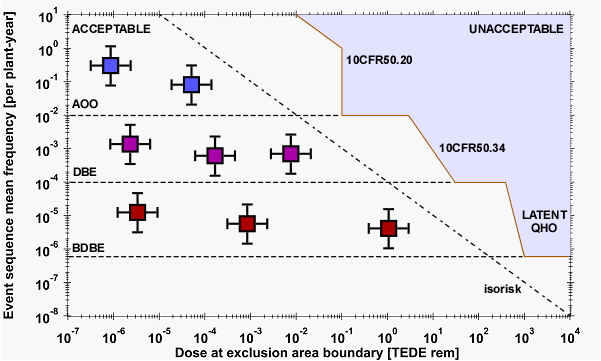
\includegraphics[width=0.85\textwidth]{farmer.jpg}
%        \caption{}
    \end{figure}
\end{frame}


\section{Risk involves three essential questions}


\section{
    What can go wrong?\\
    How likely is it to happen?\\
    What are the consequences?
}


\section{Risk assessment}


\addtocounter{framenumber}{-3}
\begin{frame}{Risk assessment starts with identification of hazards}
    \begin{enumerate}[series=outerlist,topsep=0pt,itemsep=18pt,leftmargin=*,label=(\arabic*)]
        \item[]Characterization of an individual hazard or all identified hazards combined to complete a task
        \item[]Residual risk = level of risk remaining after controls have been implemented
        \item[]Controls are altered until the residual risk is at an acceptable level or until it cannot practically be further reduced
        \item[]Multiple hazards have varying residual risk
        \item[]Kind of like \acs{ala} in nuclear engineering problems
    \end{enumerate}
\end{frame}


\begin{frame}{Risk assessment is a retrospective process}
    \begin{enumerate}[series=outerlist,topsep=0pt,itemsep=11pt,leftmargin=*,label=(\arabic*)]
        \item[]Developed by the US Space Program in 50s and 60s
        \item[]\acf{fma} to both correct missile and rocket failures
        \item[]Reactor Safety Study \href{https://uidaho.pressbooks.pub/riskassessment/chapter/pra-2/}{WASH-1400}
        \item[]Only after about 75 \acsp{npp} designed, built, operating
        \item[]First real \acs{pra} analysis
        \item[]Came to prominence after Three Mile Island in 1979
        \item[]Limited number of plant specific \acsp{pra}
        \item[]\href{https://www.nrc.gov/reading-rm/doc-collections/nuregs/staff/sr1150/}{Severe Accident Risks: An Assessment for Five U.S. Nuclear Power Plants}
        \item[]First Level III full scope \acs{pra}
    \end{enumerate}
\end{frame}


\begin{frame}{Level III assessments now done all the time to obtain operating license}
    \begin{enumerate}[series=outerlist,topsep=0pt,itemsep=15pt,leftmargin=*,label=(\arabic*)]
        \item[]\acs{nrc} paradigm now `Risk-Informed Decision Making'
        \item[]Risk assessment as one input into design and operational changes
        \item[]Deterministic and reductionistic
        \item[]Highly dependent on detailed system analysis
        \item[]Data driven and now big big data is a big big thing 
        \item[]Unless you have no operational data cohorts like for pyroprocessing or cybersecurity
    \end{enumerate}
\end{frame}


\section{Where is risk assessment used?}


\addtocounter{framenumber}{-1}
\begin{frame}{Literally everywhere}
    \begin{enumerate}[series=outerlist,topsep=0pt,itemsep=11pt,leftmargin=*,label=(\arabic*)]
        \item[]Reactor safety  
        \item[]Space shuttle
        \item[]Superfund sites
        \item[]Insurance and banking
        \item[]Information technology
        \item[]Cyber-physical systems
        \item[]Gambling and counting cards
        \item[]Finding an apartment [analytical hierarchy procedure] 
        \item[]Finding my house  
        \item[]Deciding what dessert to have
    \end{enumerate}
\end{frame}


\begin{frame}{Risk assessment contains several complex elements}
    \begin{enumerate}[series=outerlist,topsep=0pt,itemsep=15pt,leftmargin=*,label=(\arabic*)]
        \item[]Probabalistic risk assessment -- risks imposed by technologies
        \item[]Models needed due to lack of data (assumptions)
        \item[]Risk/benefit -- are the risks acceptable  
        \item[]Involuntary v voluntary
        \item[]Option generation -- risk reduction  
        \item[]Cost/benefit \& value/impact -- evaluate options
        \item[]Typically greatest good for less cost
        \item[]How much will society pay to reduce risk  
    \end{enumerate}
\end{frame}


\begin{frame}{Risk assessment is people-centered}
    \begin{enumerate}[series=outerlist,topsep=0pt,itemsep=1pt,leftmargin=*,label=(\arabic*)]
        \item[]\textbf{Public health risk analysis}
        \item[]Determination of toxic material required to cause effect
        \item[]Determination of the amount of exposure to the toxin
            \vspace{0.15in}
        \item[]\textbf{Environmental risk}
        \item[]Location and strength of source  
        \item[]Dispersion
        \item[]Uptake
        \item[]Dose + effects + response = Health effects  
        \item[]Population demographic at risk  
    \end{enumerate}
\end{frame}


\begin{frame}{Most assessments focus on acute fatalities and cancer deaths}
    \begin{enumerate}[series=outerlist,topsep=0pt,itemsep=21pt,leftmargin=*,label=(\arabic*)]
        \item[]Somatic effects = manifested in exposed individuals
        \item[]Genetic effects = manifested in exposed individuals progeny
        \item[]Deterministic effects = Severity proportional to dose
        \item[]Stochastic effects = Incident rate of exposure proportional to dose
    \end{enumerate}
\end{frame}


\begin{frame}{Risk analysis involves both technical and institutional issues}
    \begin{enumerate}[series=outerlist,topsep=0pt,itemsep=15pt,leftmargin=*,label=(\arabic*)]
        \item[]What are the risks? (assessment) -- technical
        \item[]Are the risks acceptable? -- institutional, societal context, regulations
        \item[]Can the risks be reduced? -- (options) both but more technical
        \item[]Evaluation of the options (risk/benefit, \acs{pra}) -- technical
        \item[]But the decisions (management) based on the \acs{pra} are institutional
        \item[]Because we're engineers here, we have to be technical experts
    \end{enumerate}
\end{frame}


\section{Classifying risk}


\section{The event doesn't care about society\\
         But the consequences are societal
}


\section{Severity classified by varying degrees}


\addtocounter{framenumber}{-3}
\begin{frame}{CATASTROPHIC (I)}
    \begin{enumerate}[series=outerlist,topsep=0pt,itemsep=15pt,leftmargin=*,label=(\arabic*)]
        \item[]Loss of ability to accomplish the mission or mission failure
        \item[]Death or permanent total disability (accident risk)
        \item[]Loss of major or mission-critical system or equipment
        \item[]Major property (facility) damage
        \item[]Severe environmental damage
        \item[]Mission-critical security failure 
        \item[]Unacceptable collateral damage
    \end{enumerate}
\end{frame}


\begin{frame}{CRITICAL (II)}
    \begin{enumerate}[series=outerlist,topsep=0pt,itemsep=15pt,leftmargin=*,label=(\arabic*)]
        \item[]Significantly (severely) degraded mission capability or unit readiness
        \item[]Permanent partial disability, temporary total disability exceeding 3 months time (accident risk)
        \item[]Extensive (major) damage to equipment or systems
        \item[]Significant damage to property or the environment
        \item[]Security failure
        \item[]Significant collateral damage
    \end{enumerate}
\end{frame}


\begin{frame}{MARGINAL (III)}
    \begin{enumerate}[series=outerlist,topsep=0pt,itemsep=21pt,leftmargin=*,label=(\arabic*)]
        \item[]Degraded mission capability or unit readiness
        \item[]Minor damage to equipment or systems, property, or the environment
        \item[]Lost day due to injury or illness not exceeding 3 months (accident risk)
        \item[]Minor damage to property or the environment
    \end{enumerate}
\end{frame}


\begin{frame}{NEGLIGIBLE (IV)}
    \begin{enumerate}[series=outerlist,topsep=0pt,itemsep=21pt,leftmargin=*,label=(\arabic*)]
        \item[]Little or no adverse impact on mission capability
        \item[]First aid or minor medical treatment (accident risk)
        \item[]Slight equipment or system damage, but fully functional and serviceable
        \item[]Little or no property or environmental damage
    \end{enumerate}
\end{frame}


\section{Risk matrix}


\addtocounter{framenumber}{-1}
\begin{frame}{}
    \begin{figure}
        \centering
        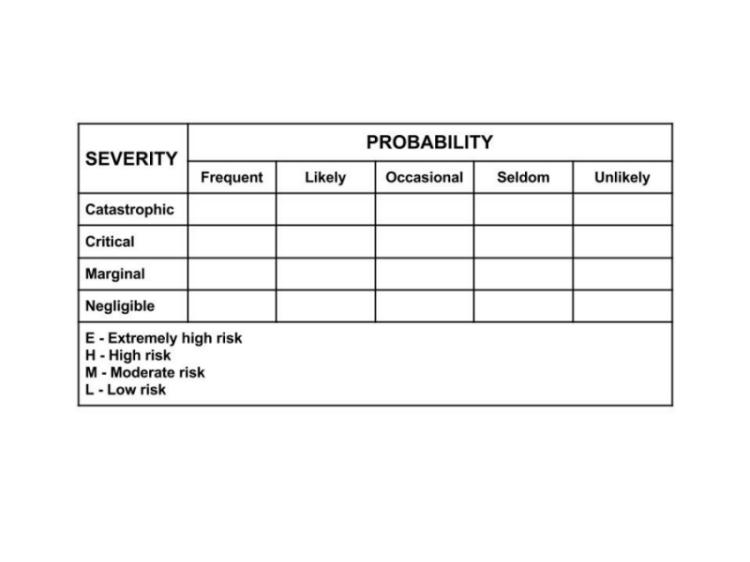
\includegraphics[width=0.85\textwidth]{risk.assessment.matrix.jpg}
%        \caption{}
    \end{figure}
\end{frame}


\begin{frame}{}
    \begin{longtable}{|c|c|c|c|c|c|}
        \hline
        \multirow{2}{*}{\textbf{Severity}} 
        & \multicolumn{5}{c|}{\textbf{Probability}} 
        \\ 
        \cline{2-6}
         
        & Frequent 
        & Likely 
        & Occasional 
        & Seldom 
        & Unlikely 
        \\ 
        \hline
        \textbf{Catastrophic} 
        & E 
        & E 
        & H 
        & H 
        & M 
        \\ 
        \hline
        \textbf{Critical}     
        & E 
        & E 
        & H 
        & M 
        & L 
        \\ 
        \hline
        \textbf{Marginal}     
        & H 
        & M 
        & M 
        & L 
        & L 
        \\ 
        \hline
        \textbf{Negligible}   
        & M 
        & L 
        & L 
        & L 
        & L 
        \\ 
        \hline
        \hline
        \multicolumn{3}{|l}{E -- Extreme Risk} 
        & \multicolumn{3}{l|}{M -- Moderate Risk} 
        \\
        \multicolumn{3}{|l}{H -- High Risk}    
        & \multicolumn{3}{l|}{L -- Low Risk} 
        \\ 
        \hline
    \end{longtable}
\end{frame}


\section{Risk management}


\addtocounter{framenumber}{-1}
\begin{frame}{Any engineering problem is inherently risk-based}
    \begin{enumerate}[series=outerlist,topsep=0pt,itemsep=21pt,leftmargin=*,label=(\arabic*)]
        \item What are the risks imposed by human activities and natural phenomena on society and the environment?
        \item Are these risks acceptable? (regulations)
        \item What are there options for reducing these risks?
        \item On what basis should we choose among these options?
    \end{enumerate}
\end{frame}


\begin{frame}{Risk management answers these questions}
    \begin{enumerate}[series=outerlist,topsep=0pt,itemsep=21pt,leftmargin=*,label=(\arabic*)]
        \item[]Process of identifying, assessing, and controlling risks arising from operational factors and making decisions that balance risk costs with mission benefits 
        \item[]Integrating risk management into mission planning, preparation, and execution
        \item[]Making risk decisions at the appropriate level in the chain of command
        \item[]Accepting no unnecessary risk
        \item[]Risk-informed, performance based decision making as part of design process
    \end{enumerate}
\end{frame}


\begin{frame}{Risk management is the process of identifying, controlling hazards to conserve combat resources}
    \begin{enumerate}[series=outerlist,topsep=0pt,itemsep=11pt,leftmargin=*,label=(\arabic*)]
        \item[]Identify hazards to people, property, mission  
        \item[]Past, present, future  
        \item[]Complexity and difficulty of the mission/task  
        \item[]Terrain and environment  
        \item[]Weather and visibility  
        \item[]Equipment on hand and status 
        \item[]Time available for preparation/execution  
        \item[](Supervision, Experience, Training, Morale, Environment)
    \end{enumerate}
\end{frame}


\section{Hazard assessment}


\addtocounter{framenumber}{-1}
\begin{frame}{Assess hazards to determine risks}
    \begin{enumerate}[series=outerlist,topsep=0pt,itemsep=11pt,leftmargin=*,label=(\arabic*)]
        \item[]Defense in depth   
        \item[]Multiple barriers
        \item[]Eliminate common failure modes (huge problem)
        \item[]Safety margins to account for uncertainty
        \item[]Develop controls  
        \item[]Implement controls  
        \item[]Supervise and evaluate  
        \item[]Risk assessment establishes situational awareness  
        \item[]Management also cost/benefit analysis
    \end{enumerate}
\end{frame}


\begin{frame}{Leaders continuously assess the risk to the overall mission and to those involved in the task}
    \begin{enumerate}[series=outerlist,topsep=0pt,itemsep=21pt,leftmargin=*,label=(\arabic*)]
        \item[]Evaluate the effectiveness of controls
        \item[]Provide lessons learned
    \end{enumerate}
\end{frame}


\section{Human factors}


\addtocounter{framenumber}{-1}
\begin{frame}{Risk assessment also involves human factors}
    \begin{enumerate}[series=outerlist,topsep=0pt,itemsep=21pt,leftmargin=*,label=(\arabic*)]
        \item[]In many cases a system being analyzed has very deterministic failures associated with it 
        \item[]Which is where we get \acs{pra}
        \item[]In reality, system failures are never well identified and humans and the organizations we create change the failure rates of systems
        \item[]And we have to live with a lot of uncertainty
    \end{enumerate}
\end{frame}


\section{Lifecycle assessment}


\addtocounter{framenumber}{-1}
\begin{frame}{Risk assessment should start early in life cycle and continue}
    \begin{enumerate}[series=outerlist,topsep=0pt,itemsep=15pt,leftmargin=*,label=(\arabic*)]
        \item[]\acf{pha} early
        \item[]\acf{fma} and fault tree analysis for conceptual design phases
        \item[]Probabilistic risk assessment and human reliability analysis for mature designs
        \item[]Continuing after system is real and is ongoing
        \item[]Nuclear reactors, technical specifications, performance goals
        \item[]Always after accidents
    \end{enumerate}
\end{frame}


\begin{frame}{}
    \begin{figure}
        \centering
        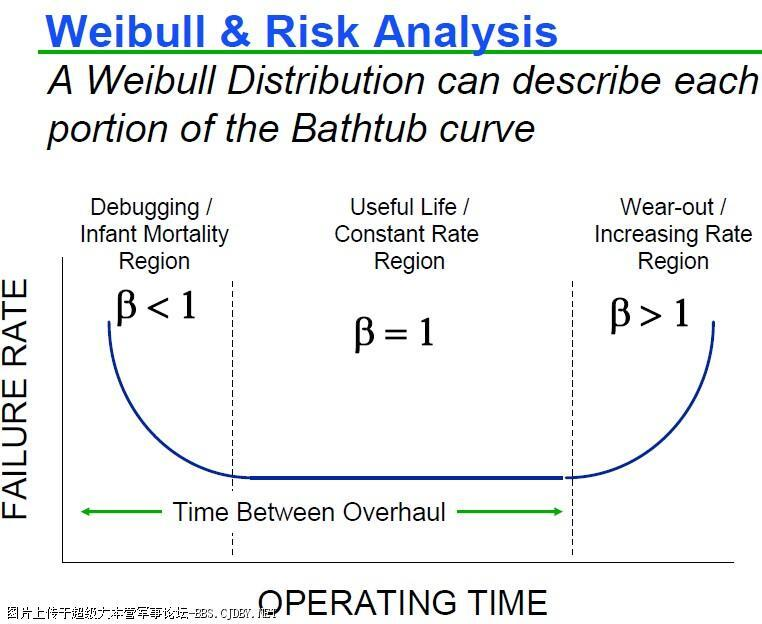
\includegraphics[width=0.75\textwidth]{bath.jpg}
%        \caption{}
    \end{figure}
\end{frame}


\begin{frame}{A Weibull distribution can describe each part of the curve}
    \begin{enumerate}[series=outerlist,topsep=0pt,itemsep=3pt,leftmargin=*,label=(\arabic*)]
        \item[]$\beta < 1$
        \item[]No operational experience or real data cohort
        \item[]Would want to minimize time period with extensive testing and modeling
            \vspace{0.10in}
        \item[]$\beta = 1$
        \item[]Random failures
            \vspace{0.10in}
        \item[]$\beta > 1$  
        \item[]So you want to know when you are heading in to here and make decisions about when to replace parts, equipment, etc.
            \vspace{0.10in}
        \item[]$Q(t) = 1 - e^{-(\frac{t}{\eta})^{\beta}}$
    \end{enumerate}
\end{frame}


\section{Frequency is not intuitive}


\addtocounter{framenumber}{-1}
\begin{frame}{Monty Hall problem}
    \begin{enumerate}[series=outerlist,topsep=0pt,itemsep=15pt,leftmargin=*,label=(\arabic*)]
        \item[]You're given the choice of three doors -- Behind one door is a car; behind the others, goats
        \item[]You pick a door; 1, and the host, who knows what's behind the doors, opens another door; 3, which has a goat
        \item[]Do you want to switch and pick door 2? Or stay with 1?
        \item[]Is it to your advantage to switch your choice? What is the probability?
        \item[]When assessing frequency, intuition can be problematic
    \end{enumerate}
\end{frame}


\begin{frame}{No spin Russian roulette}
    \begin{enumerate}[series=outerlist,topsep=0pt,itemsep=3pt,leftmargin=*,label=(\arabic*)]
        \item[]Important to fully characterize risk and understand the real problem
            \vspace{0.10in}
        \item[]\textbf{What could go wrong?}
        \item[]You have to shoot the gun
            \vspace{0.10in}
        \item[]\textbf{How likely is it to happen?}
        \item[]These are `dependent events' not like the NCAA tourney
        \item[]Because we are dependent on the chamber state AND player state
            \vspace{0.10in}
        \item[]\textbf{What are the consequences?}
        \item[]Gun goes off, you die; slow singing, flower bringing
            \vspace{0.10in}
        \item[]\textbf{Management options}
        \item[]Where should you sit to maximize you chance at life?
    \end{enumerate}
\end{frame}


\begin{frame}{Risk is the \href{https://uidaho.pressbooks.pub/riskassessment/chapter/statistical-moments/}{expected value} of an undesirable event}
    \begin{equation}
        \LARGE
        E[X] \equiv \int xf(x)dx
    \end{equation}

    \begin{equation}
        \LARGE
        E[X] \equiv \sum_i x_i f(x_i)
    \end{equation}

    \vspace*{\fill}

    \begin{enumerate}[series=outerlist,topsep=0pt,itemsep=21pt,leftmargin=*,label=(\arabic*)]
        \item[]This is the quantitative part of the risk analysis
        \item[]Not always so easy due to uncertainties
        \item[]E[DICE] = ?
    \end{enumerate}
\end{frame}


\section{Uncertainty}


\addtocounter{framenumber}{-1}
\begin{frame}{\href{https://uxdesign.cc/the-knowns-and-unknowns-framework-for-design-thinking-6537787de2c5}{Uncertainties} come in different flavors but are essential in risk}
    \begin{enumerate}[series=outerlist,topsep=0pt,itemsep=21pt,leftmargin=*,label=(\arabic*)]
        \item[]There are things we know we know
        \item[]Then there’s things we know that we do not know
        \item[]But there’s still things that we don’t know we don’t know
    \end{enumerate}
\end{frame}


\begin{frame}{Aleatory uncertainty is statistical}
    \begin{enumerate}[series=outerlist,topsep=0pt,itemsep=21pt,leftmargin=*,label=(\arabic*)]
        \item[]Random variations and chance outcomes in the physical world, natural randomness in a process
        \item[]If a parameter sometimes has one value and sometimes has another values
    \end{enumerate}
\end{frame}


\begin{frame}{Epistemic uncertainty is systematic}
    \begin{enumerate}[series=outerlist,topsep=0pt,itemsep=21pt,leftmargin=*,label=(\arabic*)]
        \item[]Lack of knowledge about the physical world, scientific uncertainty in the model of the process
        \item[]If a parameter always has either one value or another, but we are not sure which
        \item[]\href{https://www.sciencedirect.com/science/article/abs/pii/S0167473008000556}{Aleatory or epistemic? Does it matter?}
    \end{enumerate}
\end{frame}


\section{Ethics}


\addtocounter{framenumber}{-1}
\begin{frame}{There is an ethical theory basis for risk}
    \begin{enumerate}[series=outerlist,topsep=0pt,itemsep=21pt,leftmargin=*,label=(\arabic*)]
        \item[]Based on universal rules and principles by Descartes (1596--1650)
        \item[]Rights ethics by John Locke (not the guy from the Island) (1632--1704)
        \item[]Duties ethics by Immanuel Kant (1724--1804)
        \item[]Utilitarianism by Jeremy Bentham and John Stuart Mill (1748--1832),(1806--1873)
        \item[]`Greatest good for greatest number of people' (Red Wedding)
        \item[]\acs{pra} (WASH1400) comes from this -- `economic determinism'; cost/benefit
    \end{enumerate}
\end{frame}


\section{Societal context}


\addtocounter{framenumber}{-1}
\begin{frame}{Society determines acceptable risks}
    \begin{enumerate}[series=outerlist,topsep=0pt,itemsep=21pt,leftmargin=*,label=(\arabic*)]
        \item[]\acf{ala} (1000/person/rem)
        \item[]Versus precautionary principle
        \item[]Contaminated [superfund] sites and cancer risks
        \item[]Safety goals for reactors, 0.1\% of background cancer risk
        \item[]So it is the regulations that determine the acceptable levels
    \end{enumerate}
\end{frame}


\begin{frame}{How is that codified?}
    \begin{enumerate}[series=outerlist,topsep=0pt,itemsep=21pt,leftmargin=*,label=(\arabic*)]
        \item[]\acs{nrc} has qualitative safety goals
        \item[]Individuals bear no significant additional risk to life and health
        \item[]Societal risks to life and health from nuclear power plant operation should be comparable to or less than the risks due to electric generation by competing technologies and should not be a significant addition to other societal risks
        \item[]There’s more, but you get the idea
    \end{enumerate}
\end{frame}


\begin{frame}{What are some examples of utilitarianism in real life?}
    \begin{enumerate}[series=outerlist,topsep=0pt,itemsep=21pt,leftmargin=*,label=(\arabic*)]
        \item[]Insurance -- How much am I willing to spend each year to insure my house, car, life and for what amount?
        \item[]Energy -- What risks am I willing to take for the benefit of 1000 MWe among a coal, natural gas, oil or nuclear power plant?
        \item[]These are not strictly technically-based? Or not?
    \end{enumerate}
\end{frame}


\begin{frame}{Cost/benefit is the typical risk reduction mode}
    \begin{enumerate}[series=outerlist,topsep=0pt,itemsep=21pt,leftmargin=*,label=(\arabic*)]
        \item[]Rational decision maker will choose the option that maximizes utility
        \item[]Or largest benefit/cost ratio
        \item[]Multiattribute utilty theory uses functions to express risk aversion
        \item[]Use of decision trees
        \item[]Relies on expert judgement
        \item[]Game theory for two party decision making
    \end{enumerate}
\end{frame}


\section{Brief case study}


\section{Challenger}


\addtocounter{framenumber}{-2}
\begin{frame}{The Challenger disaster occurred in 1986}
    \begin{enumerate}[series=outerlist,topsep=0pt,itemsep=21pt,leftmargin=*,label=(\arabic*)]
        \item[]The Space Shuttle management prior to the Challenger disaster felt that a failure would occur about 1 every 100,000 flight
        \item[]Engineers calculated the failure rates between 1 in 100 and 1 in 556 missions pre-Challenger
        \item[]In actuality the failure rates were 1 in 137 on launch and 1 in 137 on re-entry or 2 in 137 flights
        \item[]Human decision process gravely impacted the Challenger mission 
        \item[]How frequency is determined affects management options
    \end{enumerate}
\end{frame}


\section{Ford Pinto}


\addtocounter{framenumber}{-1}
\begin{frame}{The Ford Pinto case is a classic study of risk/benefit and ethics}
    \begin{enumerate}[series=outerlist,topsep=0pt,itemsep=21pt,leftmargin=*,label=(\arabic*)]
        \item[]During design and production, crash tests revealed a serious defect in the gas tank
        \item[]In crashes over \textit{25 miles per hour}, the gas tank always ruptured
        \item[]To correct it would have required changing and strengthening the design
        \item[]So they didn’t
        \item[]What other more contemporary examples are there?
    \end{enumerate}
\end{frame}


\begin{frame}{}
    \begin{figure}
        \centering
        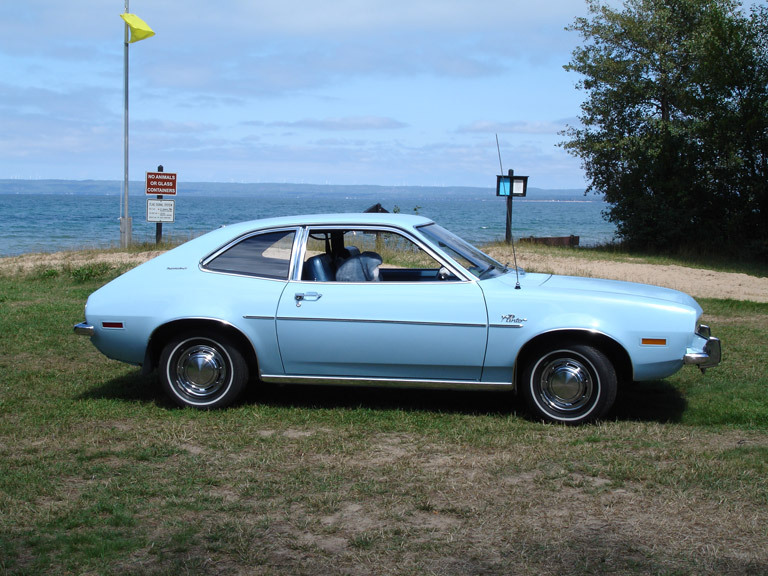
\includegraphics[width=0.75\textwidth]{blue.pinto.jpg}
%        \caption{}
    \end{figure}
\end{frame}


\begin{frame}{}
    \begin{figure}
        \centering
        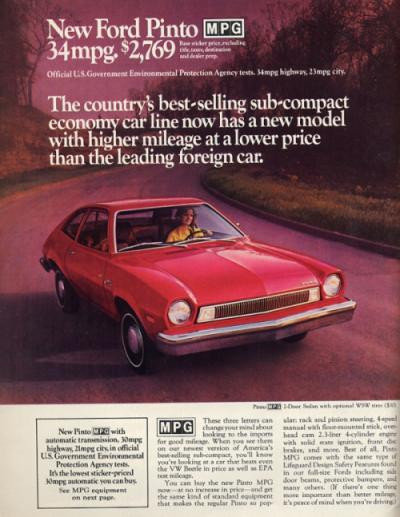
\includegraphics[width=0.45\textwidth]{pinto.ad.jpg}
%        \caption{}
    \end{figure}
\end{frame}


\begin{frame}{}
    \begin{figure}
        \centering
        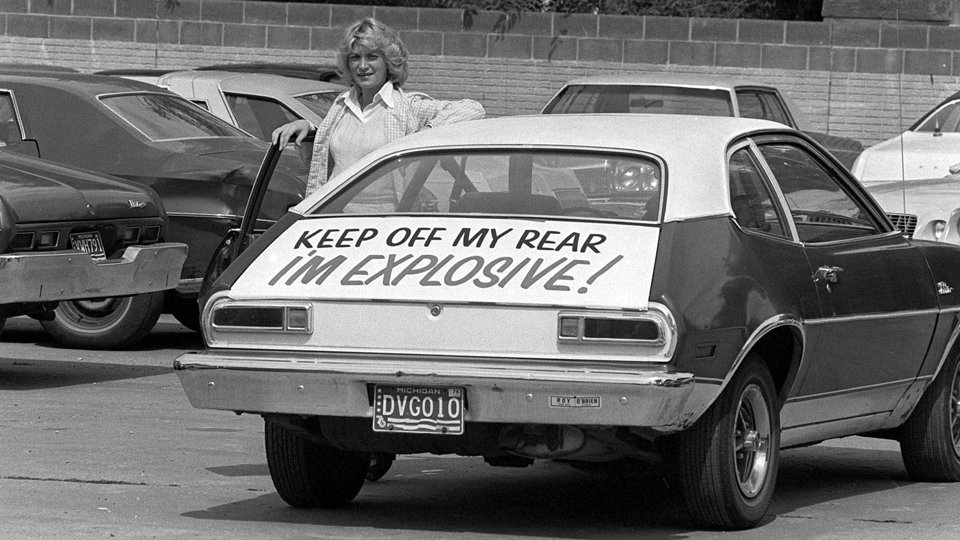
\includegraphics[width=0.75\textwidth]{pinto.rear.jpg}
%        \caption{}
    \end{figure}
\end{frame}


\begin{frame}{}
    \begin{figure}
        \centering
        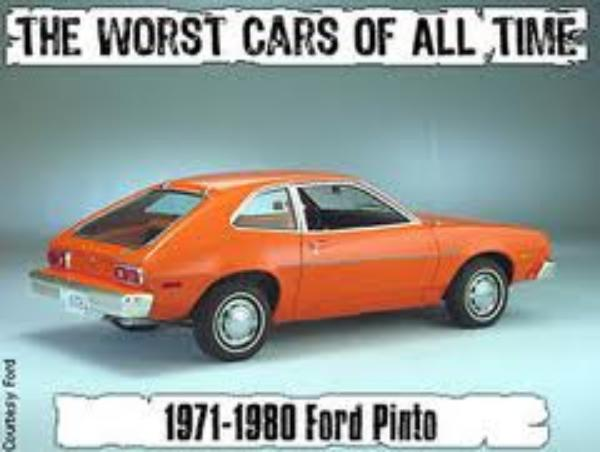
\includegraphics[width=0.75\textwidth]{pinto.worst.jpg}
%        \caption{}
    \end{figure}
\end{frame}


\begin{frame}{}
    \begin{figure}
        \centering
        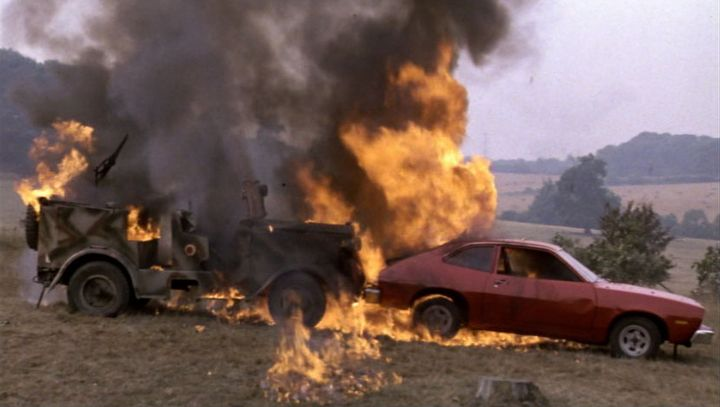
\includegraphics[width=0.75\textwidth]{pinto.fire.jpg}
%        \caption{}
    \end{figure}
\end{frame}


\section{Repository}


\addtocounter{framenumber}{-1}
\begin{frame}{How does a repository distribute risk?}
    \begin{columns}[c]

        \begin{column}{0.65\textwidth}
            \begin{figure}
                \centering
                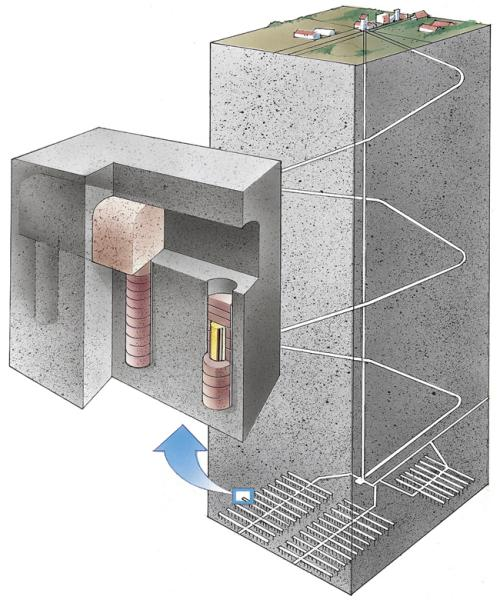
\includegraphics[width=0.65\textwidth]{kbs.jpg}
                %        \caption{}
            \end{figure}
        \end{column}

        \begin{column}{0.35\textwidth}
            \begin{enumerate}[series=outerlist,topsep=0pt,itemsep=21pt,leftmargin=*,label=(\arabic*)]
                \item[]Single location
                \item[]Greatest good for whom?
            \end{enumerate}
        \end{column}

    \end{columns}
\end{frame}


\section{\href{https://youtu.be/rvkEpstd9os}{Dreamliner}}


\addtocounter{framenumber}{-1}
\begin{frame}{}
    \begin{figure}
        \centering
        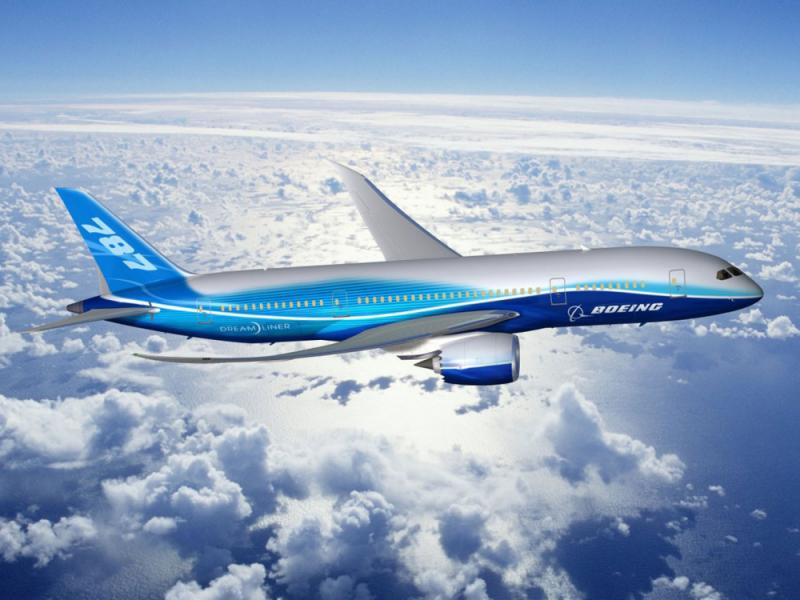
\includegraphics[width=0.75\textwidth]{dreamliner.jpg}
%        \caption{}
    \end{figure}
\end{frame}


\section{Drawbacks}


\addtocounter{framenumber}{-1}
\begin{frame}{What are some drawbacks of utilitarianism?}
    \begin{enumerate}[series=outerlist,topsep=0pt,itemsep=11pt,leftmargin=*,label=(\arabic*)]
        \item[]Only the greatest good, as a singular body and not distributed among people
        \item[]Difficulty in quantifying the greatest good
        \item[]Plus there are always lots of uncertainties to trust one number
        \item[]Anthropocentric
        \item[]Utilitarianism judges by consequences rather than actions
        \item[]Low probability--high consequence events carry as much weight as high probability--low consequence events
        \item[]Emerging technologies exhibit nonlinearity [emergent quality]
        \item[]Time scales
        \item[]Yet utilitarianism is how we do risk in everything
    \end{enumerate}
\end{frame}


\section{Alternatives}


\addtocounter{framenumber}{-1}
\begin{frame}{What else can be used?}
    \begin{enumerate}[series=outerlist,topsep=0pt,itemsep=21pt,leftmargin=*,label=(\arabic*)]
        \item[]Justice ethics by Rawls (1971)
        \item[]This is something else covered in detail in an ethics course
        \item[]Each person is to have an equal right to equal basic liberties
        \item[]Social and economic inequalities are to the greatest benefit of the least--advantaged
        \item[]Treating everyone equally is a challenge
        \item[]\href{https://www.epa.gov/environmentaljustice}{Evironmental justice}
    \end{enumerate}
\end{frame}


\section{Fault trees}


\addtocounter{framenumber}{-1}
\begin{frame}{Fault tree is a top down, deductive failure analysis tool}
    \begin{columns}[c]

        \begin{column}{0.65\textwidth}
            \begin{figure}
                \centering
                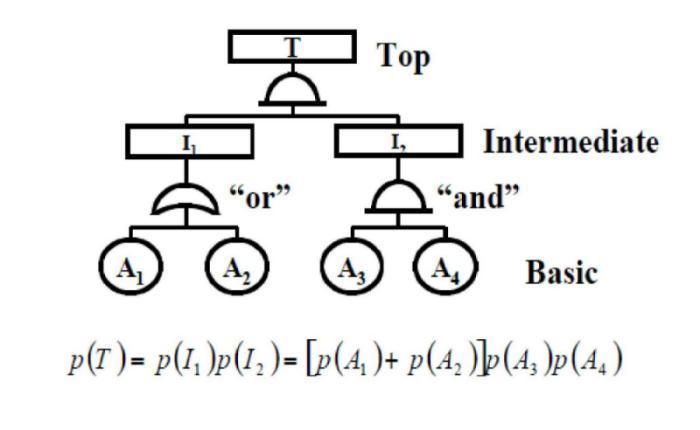
\includegraphics[width=0.65\textwidth]{fault.tree.jpg}
                %        \caption{}
            \end{figure}
        \end{column}

        \begin{column}{0.35\textwidth}
            \begin{enumerate}[series=outerlist,topsep=0pt,itemsep=21pt,leftmargin=*,label=(\arabic*)]
                \item[]Logic diagram for the system
                \item[]Top is `big system event' like \acf{loc}
            \end{enumerate}
        \end{column}

    \end{columns}
\end{frame}


\begin{frame}{}
    \begin{figure}
        \centering
        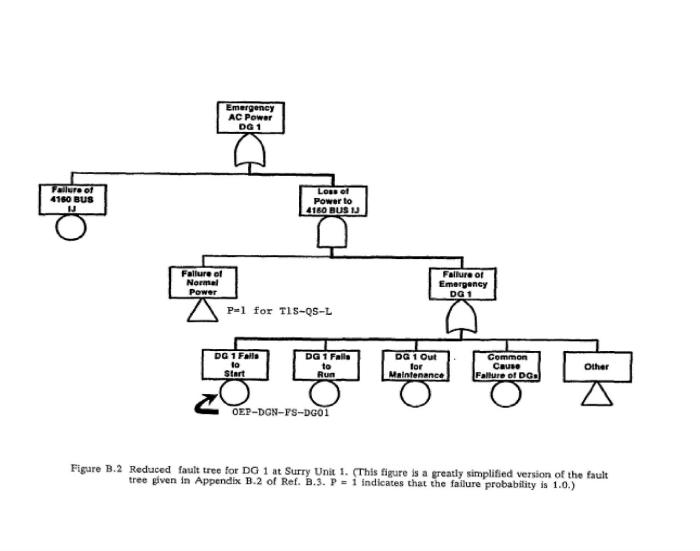
\includegraphics[width=0.75\textwidth]{fault.tree.wash.jpg}
%        \caption{}
    \end{figure}
\end{frame}


\section{Event trees}


\addtocounter{framenumber}{-1}
\begin{frame}{}
    \begin{columns}[c]

        \begin{column}{0.65\textwidth}
            \begin{figure}
                \centering
                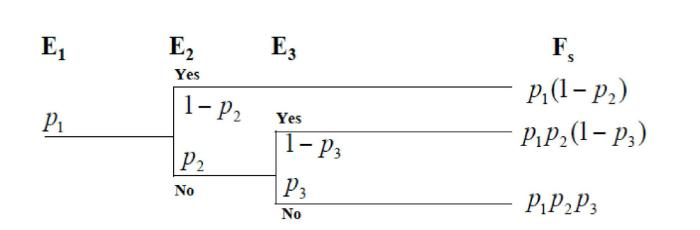
\includegraphics[width=0.65\textwidth]{event.tree.jpg}
                %        \caption{}
            \end{figure}
        \end{column}

        \begin{column}{0.35\textwidth}
            \begin{enumerate}[series=outerlist,topsep=0pt,itemsep=21pt,leftmargin=*,label=(\arabic*)]
                \item[]Consequence is associated with the final state
                \item[]Dose/response models
            \end{enumerate}
        \end{column}

    \end{columns}
\end{frame}


\begin{frame}{}
    \begin{figure}
        \centering
        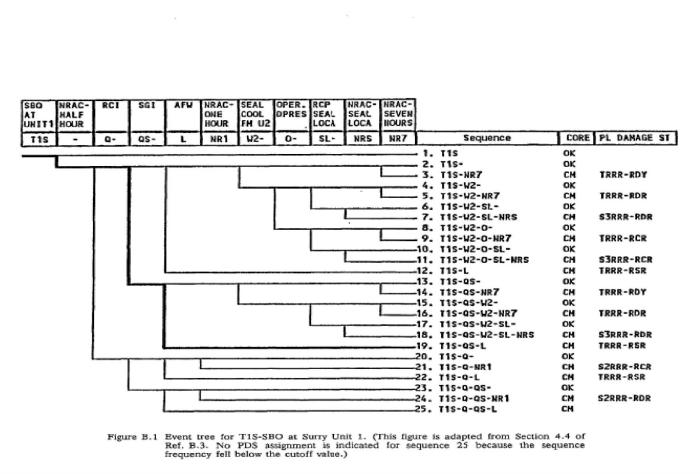
\includegraphics[width=0.75\textwidth]{event.tree.wash.jpg}
%        \caption{}
    \end{figure}
\end{frame}


\begin{frame}{}
    \begin{figure}
        \centering
        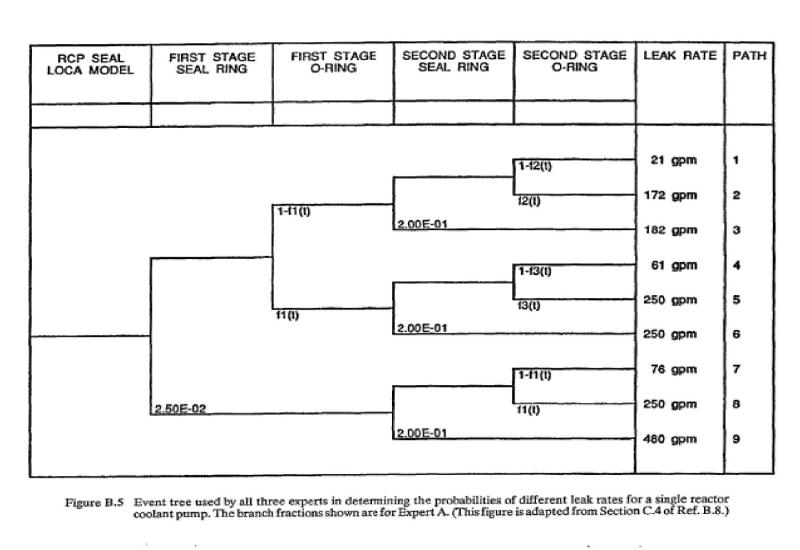
\includegraphics[width=0.75\textwidth]{event.tree.gpm.jpg}
%        \caption{}
    \end{figure}
\end{frame}


\section{Risk perception}


\addtocounter{framenumber}{-1}
\begin{frame}{Risk/benefit is just a tool, the result alone is not the decision, this requires societal context and ethics}
    \begin{enumerate}[series=outerlist,topsep=0pt,itemsep=21pt,leftmargin=*,label=(\arabic*)]
        \item[]Inherently, there is the issue of risk perception by different stakeholders
        \item[]Particularly with anything nuclear related
        \item[]Historical inertia
        \item[]Social scientists say quantification is insufficient to address risk
        \item[]Risk--informed approaches
    \end{enumerate}
\end{frame}


\begin{frame}{Risk perception is a challenge to overcome}
    \begin{figure}
        \centering
        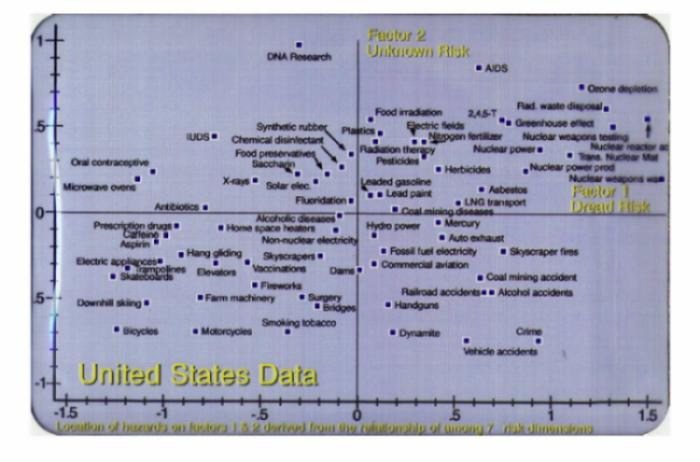
\includegraphics[width=0.75\textwidth]{risk.perception.jpg}
%        \caption{}
    \end{figure}
\end{frame}


\begin{frame}{Seminal literature}
    \begin{enumerate}[series=outerlist,topsep=0pt,itemsep=21pt,leftmargin=*,label=(\arabic*)]
        \item[]On the quantitative definition of risk
        \item[]The Hyatt Horror
        \item[]The Pinto Case
        \item[]\href{https://uidaho.pressbooks.pub/riskassessment/chapter/pra-2/}{Reactor accident scenarios -- \acs{loc}}
        \item[]\href{https://uidaho.pressbooks.pub/riskassessment/chapter/contemporary-cases-in-risk-assessment-2/}{Media}
    \end{enumerate}
\end{frame}


\begin{frame}[plain]{}
    \begin{figure}
        \centering
        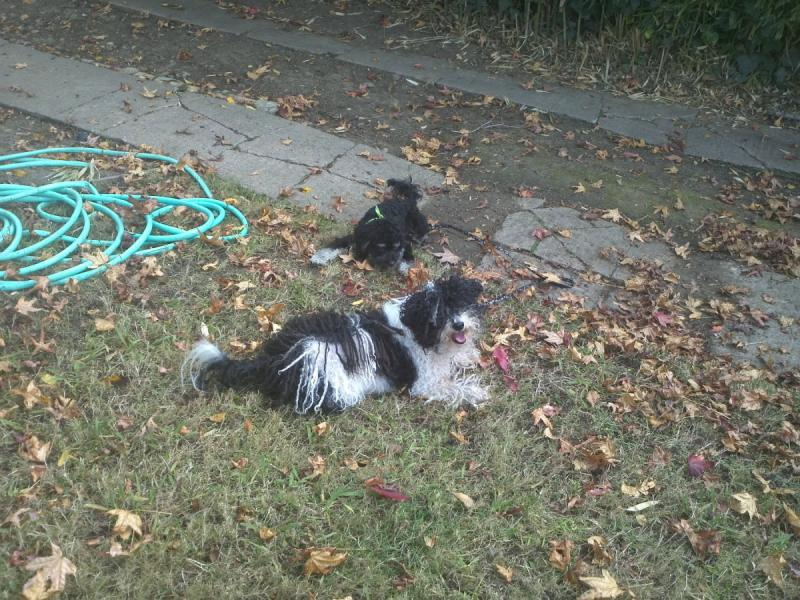
\includegraphics[width=0.65\textwidth]{final.jpg}
%        \caption{}
    \end{figure}
\end{frame}


%%%%%%%
%\begin{frame}{}
%    \begin{columns}
%
%        \begin{column}{0.50\textwidth}
%            \begin{enumerate}[series=outerlist,topsep=0pt,itemsep=21pt,leftmargin=*,label=(\arabic*)]
%                \item[]
%                \item[]
%            \end{enumerate}
%        \end{column}
%
%        \begin{column}{0.50\textwidth}
%            \begin{enumerate}[series=outerlist,topsep=0pt,itemsep=21pt,leftmargin=*,label=(\arabic*)]
%                \item[]
%                \item[]
%            \end{enumerate}
%        \end{column}
%
%    \end{columns}
%\end{frame}

%    \begin{figure}
%        \centering
%        \includegraphics[width=0.75\textwidth]{wsc.png}
%        \caption{\acs{wsc}}
%    \end{figure}


%\begin{frame}{References}
%    \bibliographystyle{nsf}
%    \footnotesize
%    \bibliography{references}
%\end{frame}
%%%%%%%


\end{document}
